%% document
\documentclass[11pt]{article}
\usepackage[letterpaper, portrait, margin=0.75in]{geometry}
\usepackage{setspace}
\usepackage{color}

% text
\usepackage[utf8]{inputenc}
\setlength\parindent{0pt}
\setlength{\parskip}{1em}
\usepackage{enumitem}
\renewcommand{\familydefault}{\sfdefault}
\newcommand{\RomanNumeral}[1]{\textrm{\uppercase\expandafter{\romannumeral #1\relax}}}

% math
\usepackage{amssymb}
\usepackage{amsmath}
\usepackage[cm]{sfmath}
\usepackage{commath}
\usepackage{multirow}
\DeclareMathAlphabet{\mathpzc}{OT1}{pzc}{m}{it}

% graphics
\usepackage{graphics}
\usepackage{graphicx}
\usepackage{epsfig}
\usepackage{epstopdf}
\usepackage{xpatch}
\usepackage{pdfpages}
\usepackage{float}

% each section begins new page
\let\stdsection\section
\renewcommand\section{\clearpage\stdsection}

% hyperref
\usepackage{hyperref}
\hypersetup{
	colorlinks,
	bookmarksopen,
	bookmarksnumbered,
	hidelinks,
}
\usepackage[all]{hypcap}  % helps hyperref work properly

% bibliography
\usepackage[numbers]{natbib}

% title
\title{Wisconsin Photoreactor \\ Assembly Instructions}
\author{
  Philip Lampkin \\
  Blaise J. Thompson \\
  Samuel H. Gellman
  }
\date{\today}

\begin{document}

\maketitle


\includegraphics[width=\textwidth]{"../coverart.jpg"}

\tableofcontents

\section{Introduction}

Throughout this document we refer to an online repository containing source and design files.
This repository appears at \url{https://github.com/uw-madison-chem-shops/wisconsin-photoreactor}.
This repository contains everything including the source for this very document.

\section{3D Printed Enclosure}

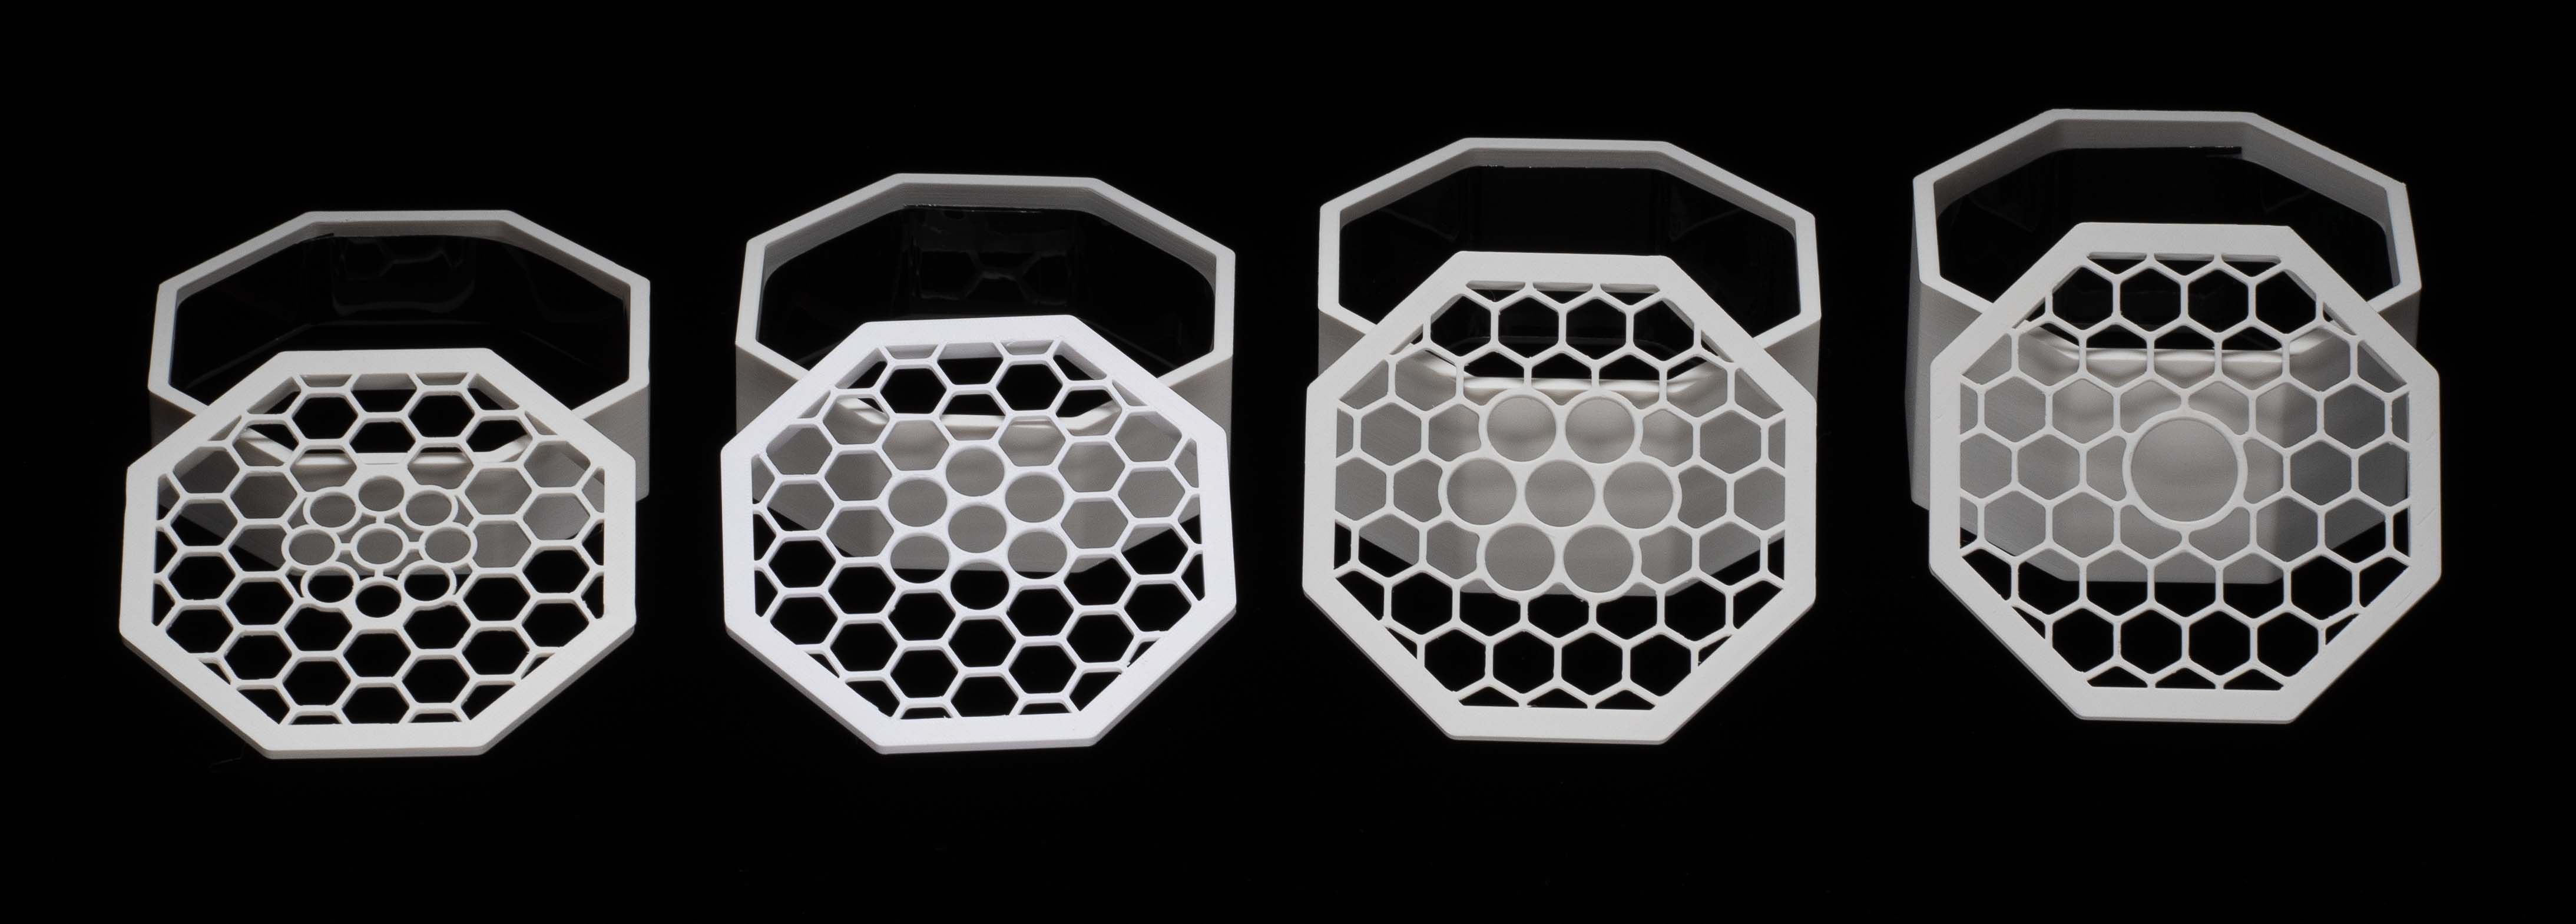
\includegraphics[width=\textwidth]{"./3dp-coverat.jpg"}

\section{Electronics}

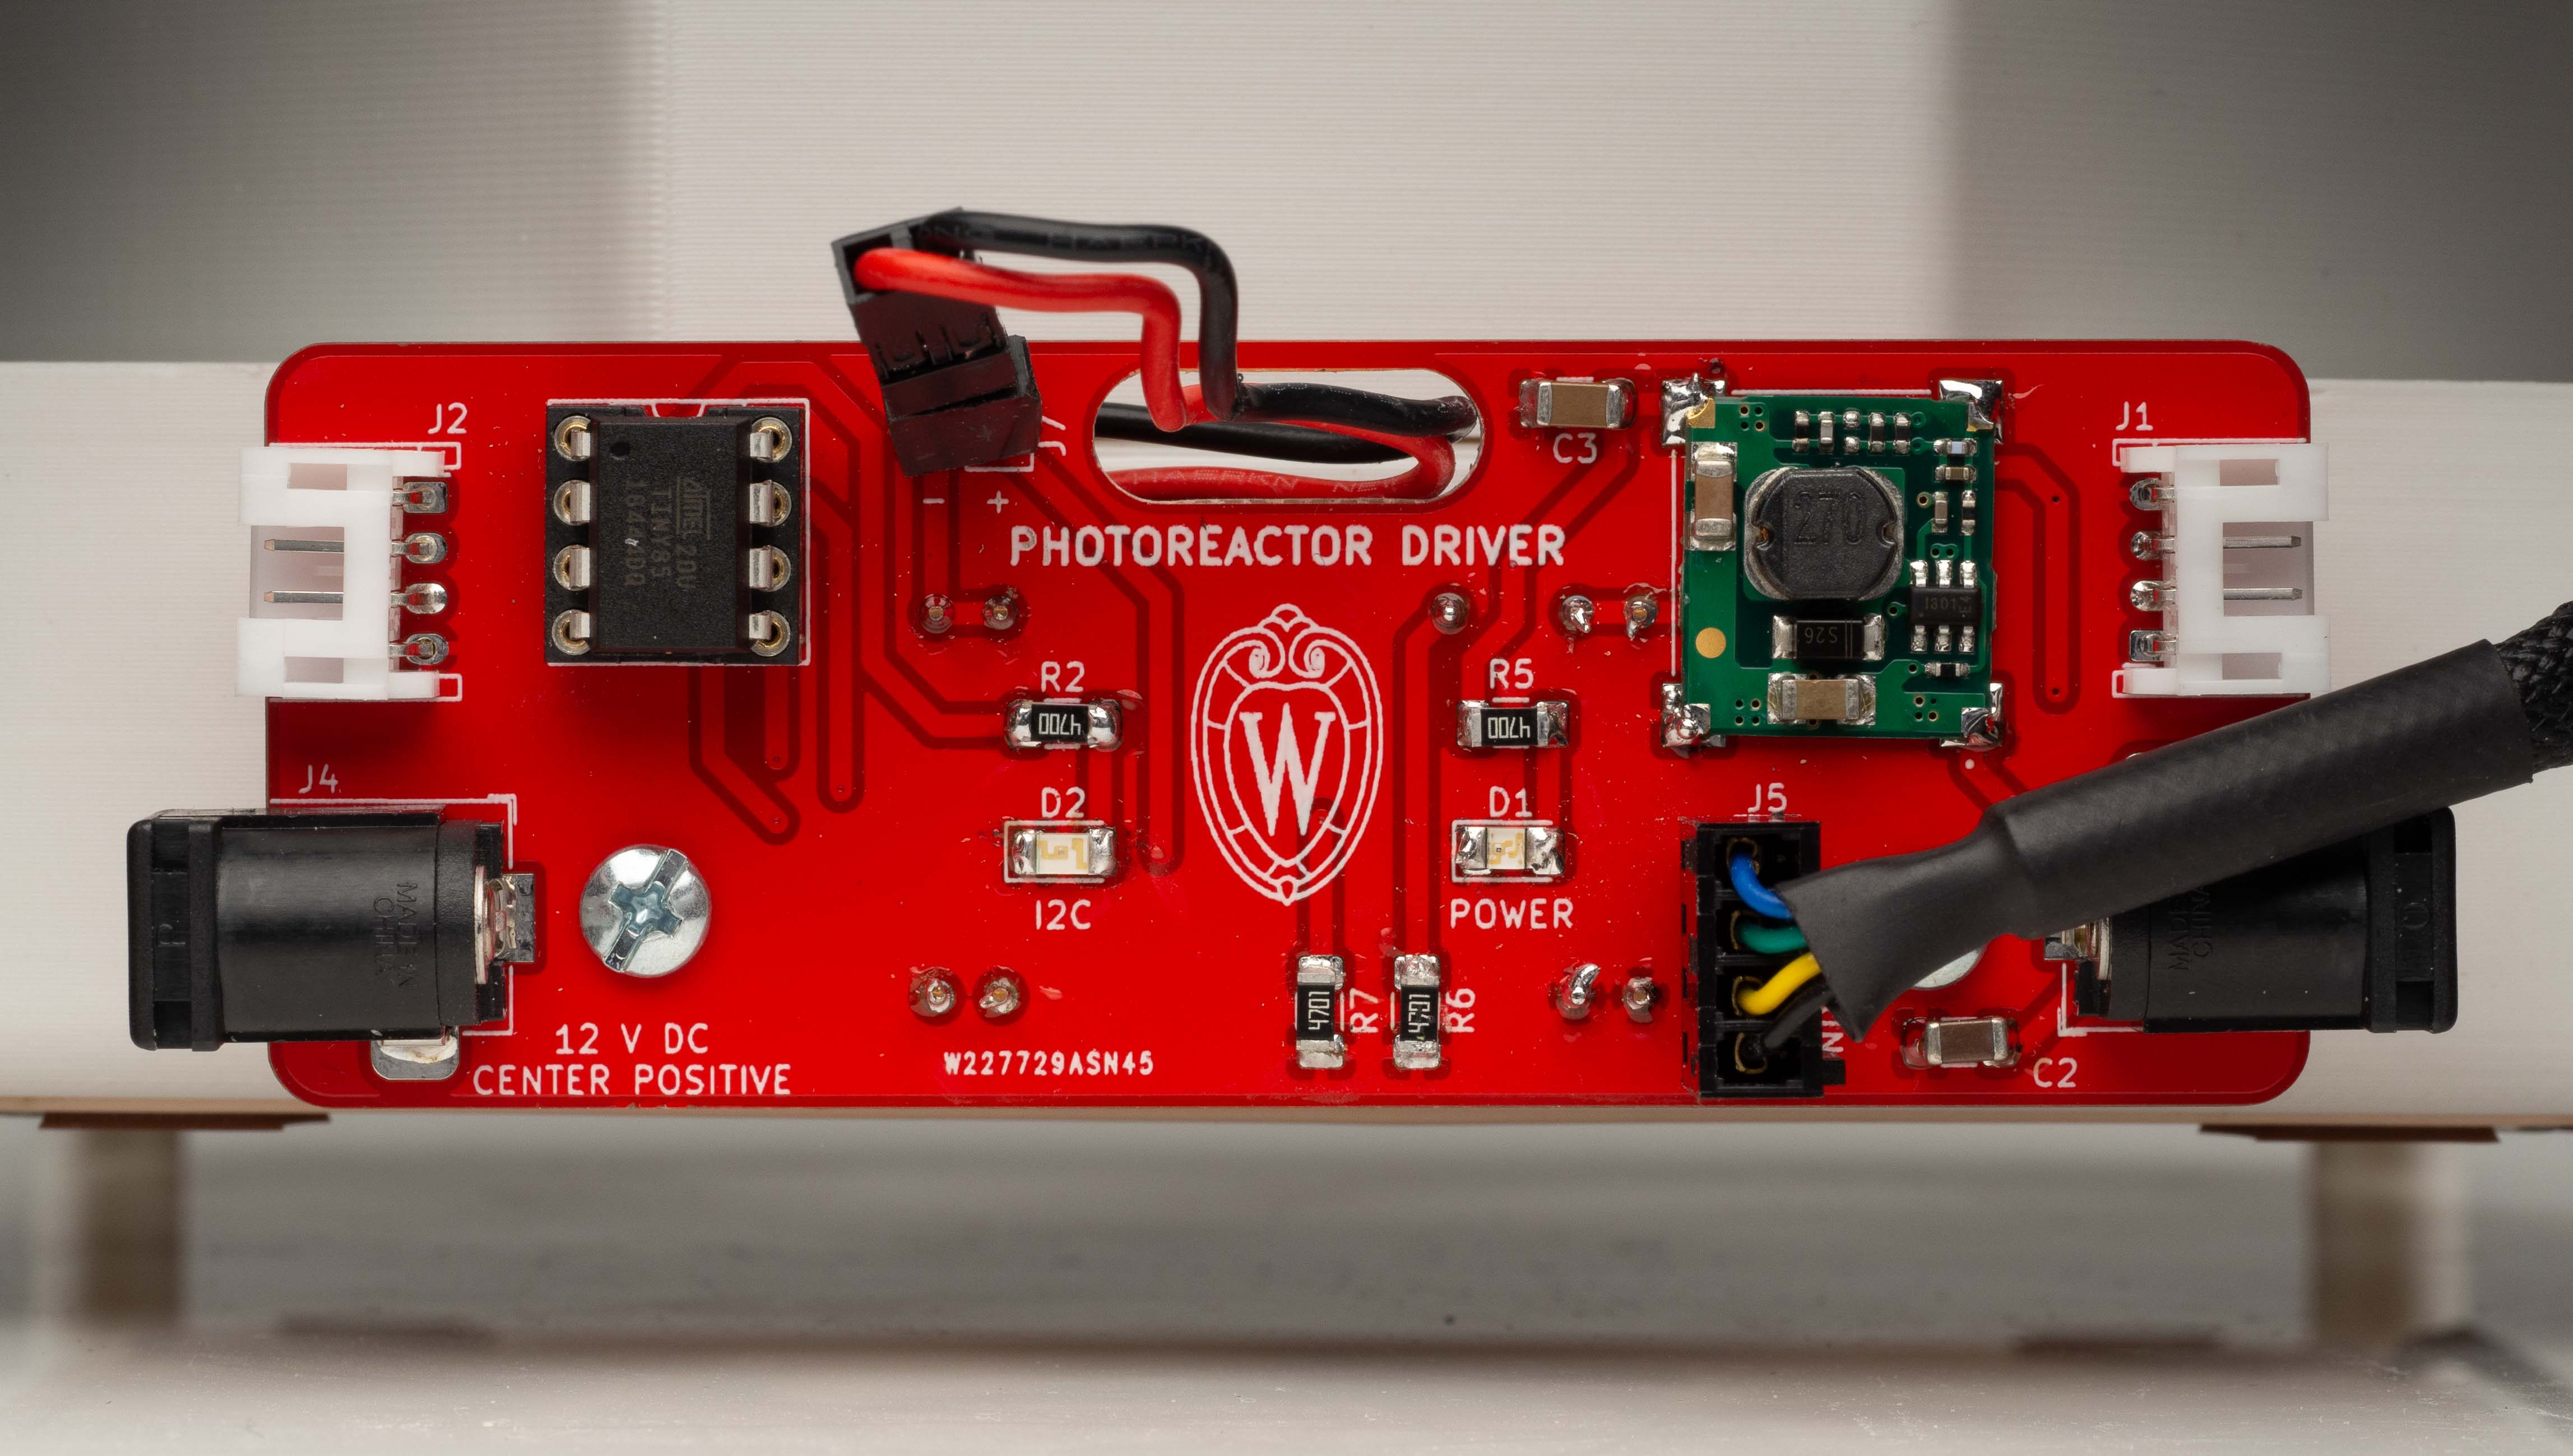
\includegraphics[width=\textwidth]{"./electronics-coverart.jpg"}

\subsection{Analog}

\includepdf[landscape=true]{"../analog-driver/driver.pdf"}

\subsection{Digital}

TODO: document I2C connection choice.
Consistent with Adafruit, Sparkfun, Seeed...

\subsubsection{Driver}

\includepdf[landscape=true]{"../digital-driver/driver.pdf"}

\subsubsection{Controller}

\section{Assembly}

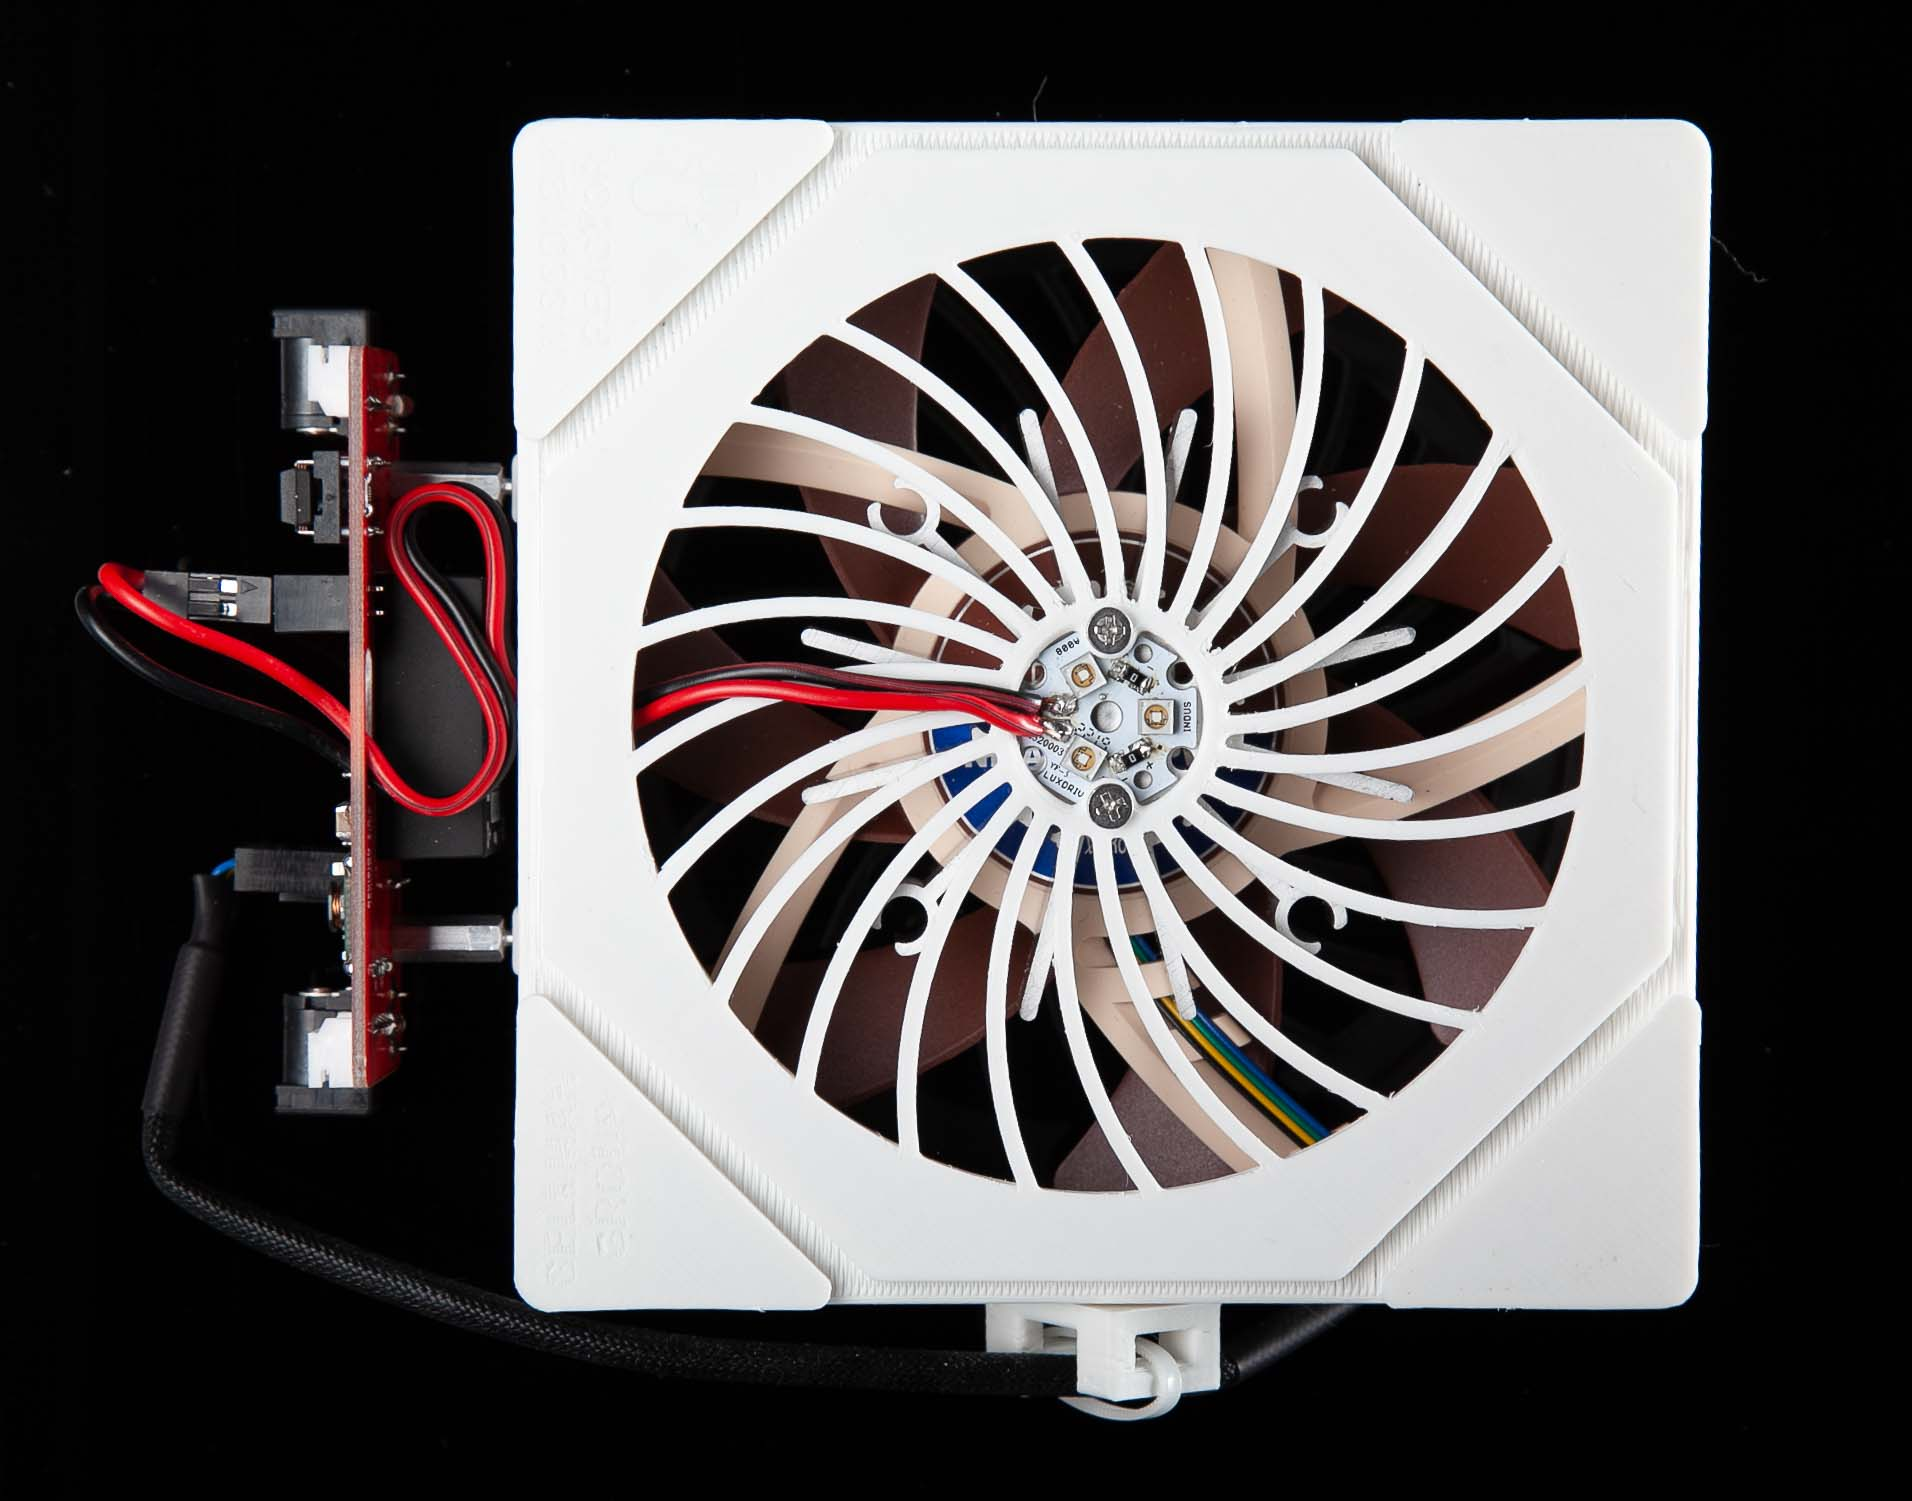
\includegraphics[width=\textwidth]{"./assembly-coverart.jpg"}


0.5'' standoff: RAF 4505-440-AL

\subsection{Base}

\subsubsection{LED and Heatsink}

TODO: LED PCB part number

TODO: heatsink part number

\begin{figure}[H]
  \centering
  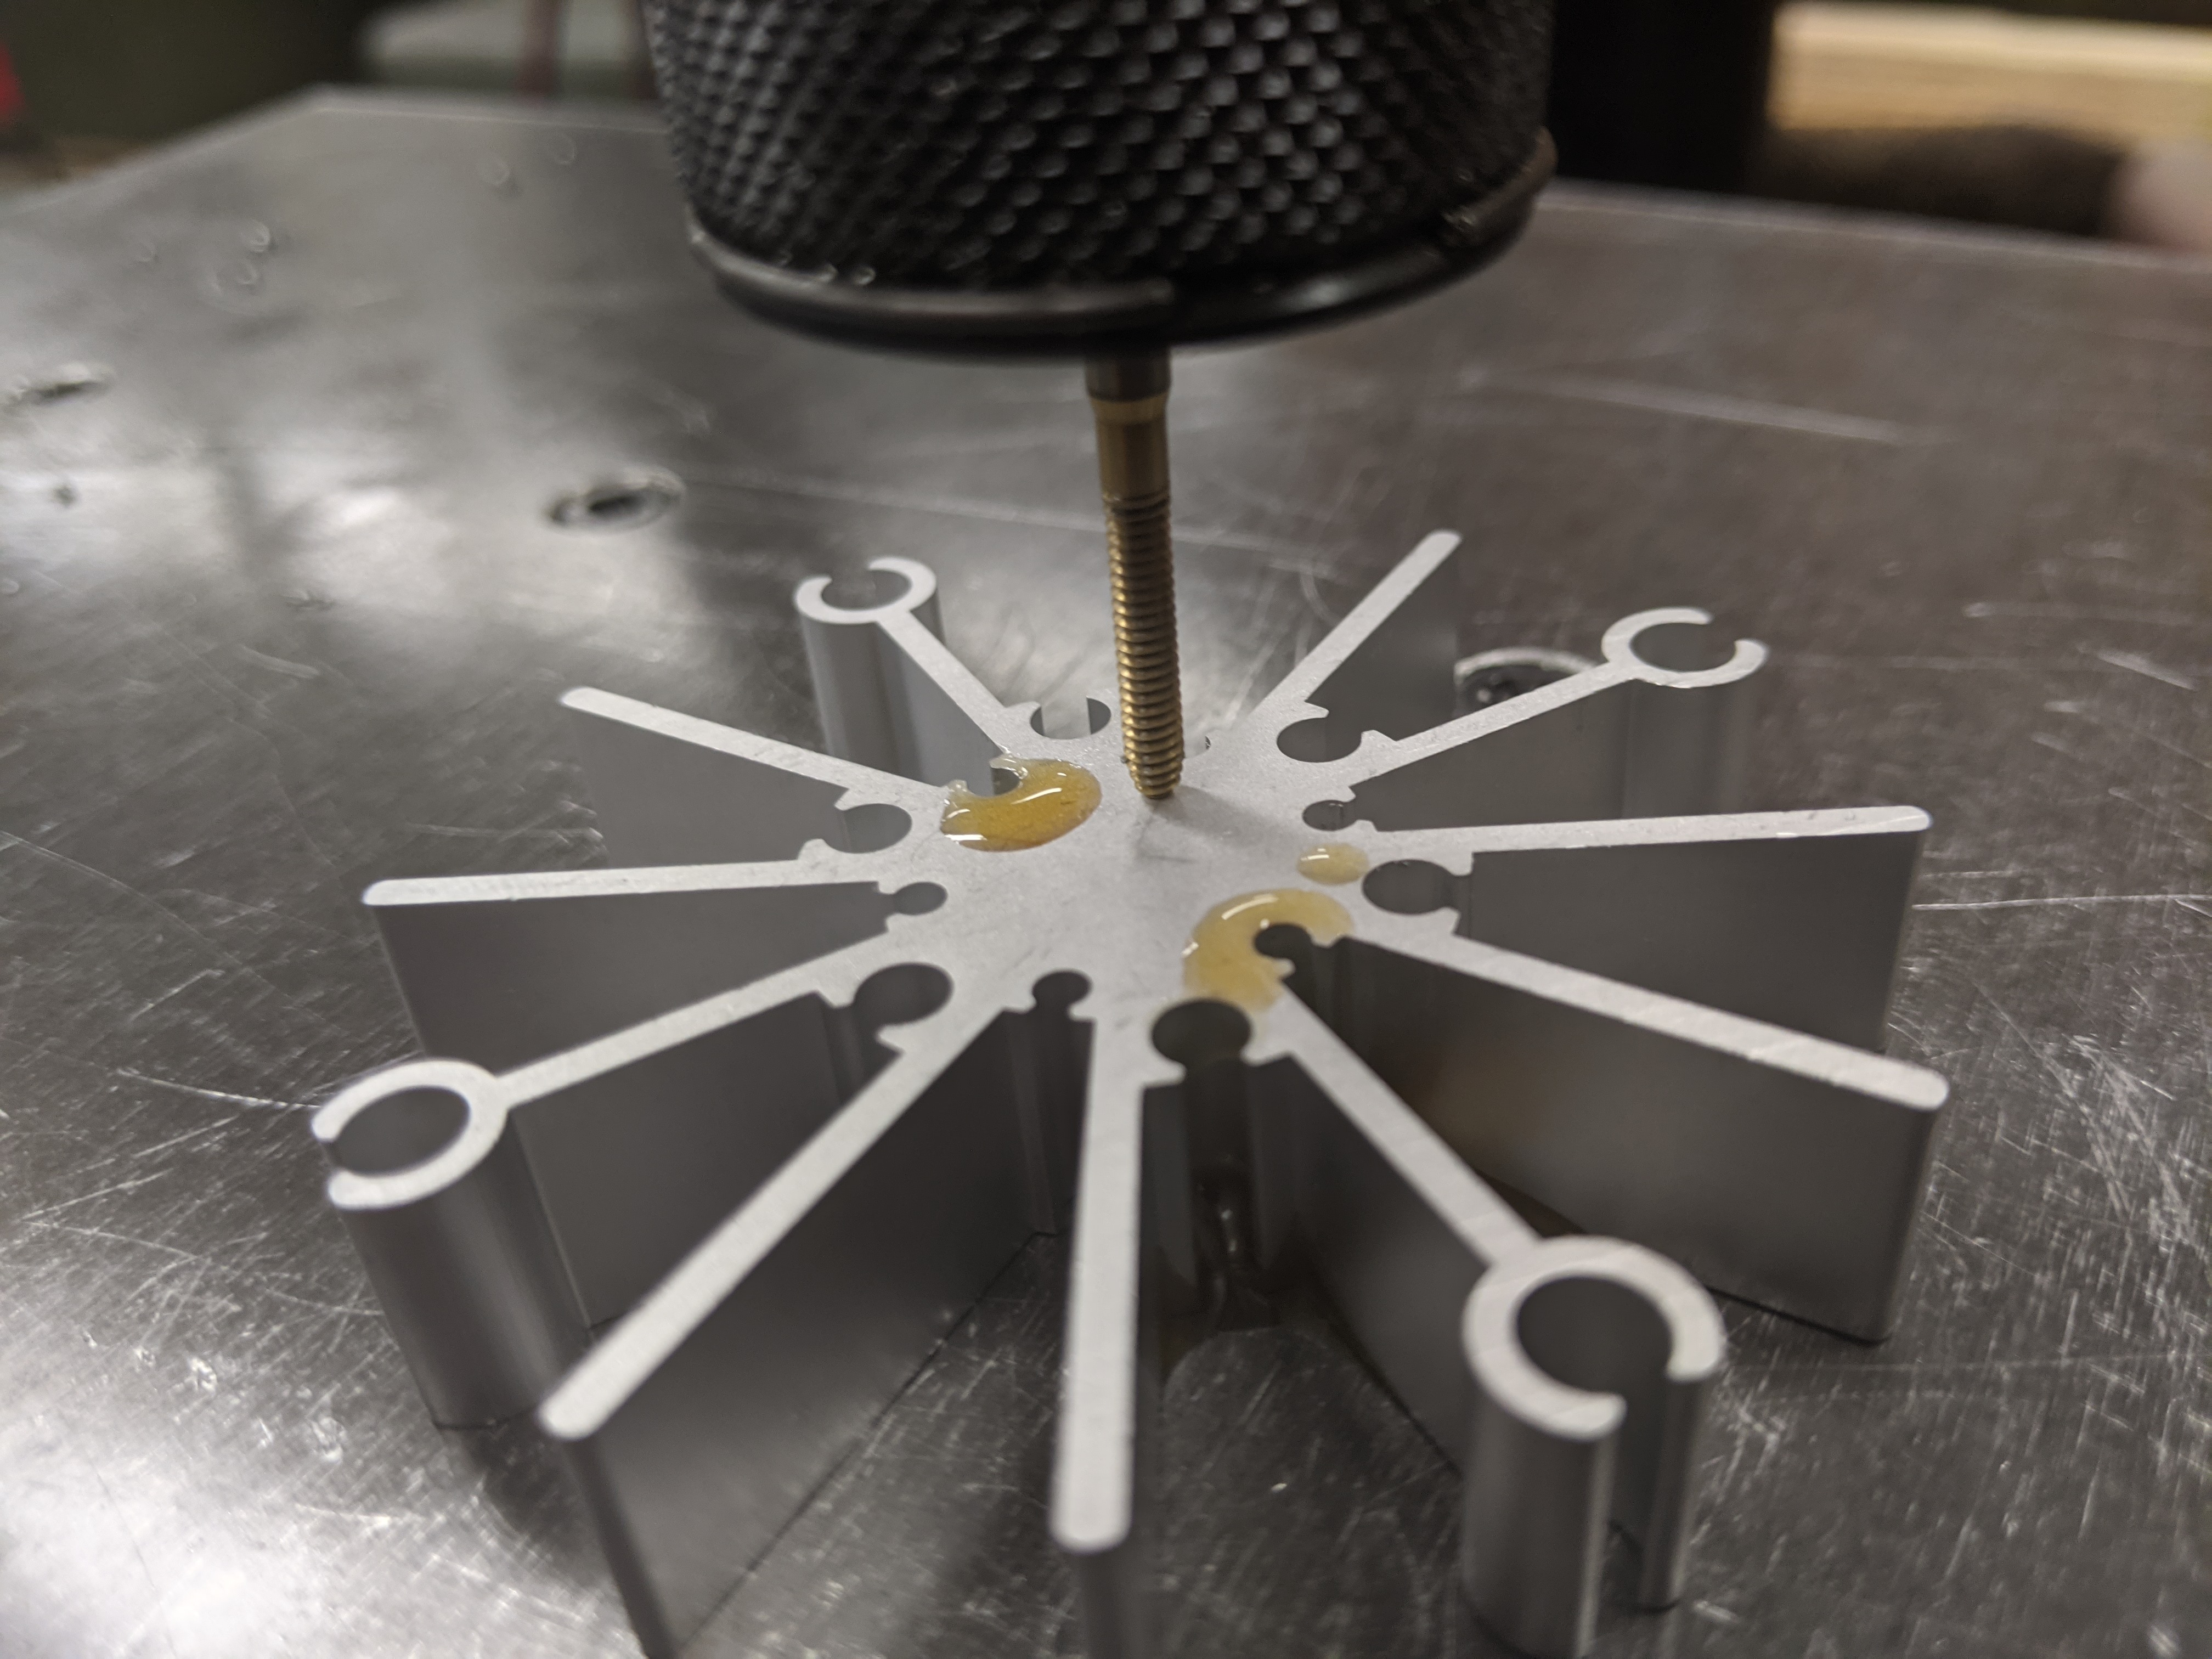
\includegraphics[width=\textwidth/2]{"./tap-heatsink.jpg"}
  \caption{Two of the innermost holes on the extruded heatsink must be 4-40 tapped.}
\end{figure}

Tap the heatsink.
We used thread-forming tap: OSG 1400105300.

TODO: heatsink compoud

Install with wires facing towards printed hole

Use 4-40 1/4''.

\subsubsection{Fan}

TODO: fan part number

Noctua NF-A12x15 PWM

pins:
blue: PWM (5 V)
yellow: +12 V
black: ground

Use 4-40 3/4'' into captured nuts

\end{document}
